\section{Filter\hartl{509}}
\subsection{Tiefpass-Filter\hartl{514}}

\subsubsection{1. Ordnung}
\begin{multicols}{2}
	\textbf{Aufbau:} \\
	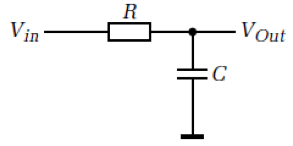
\includegraphics[scale=0.4]{pictures/tiefpass1ordnung} \\
	\textbf{UTF: } $G(s): \frac{1}{1+s\cdot C\cdot R}$ \\
	\textbf{Zeitkonstante T:} \\
	Bei $j\omega=\frac{1}{T}$ sind Real-  und Imaginärteil gleich gross:  \\
	$T=\frac{1}{R \cdot C}$ \\
	\textbf{Amplitude} $\frac{1}{1.41}\to 3dB$ : $f_{3dB}=\frac{1}{2\pi R\cdot C}$ \\	
\end{multicols}



\subsubsection{2. Ordnung}
\begin{itemize}
  \item Kaskadierte RC-Tiefpässe\\
  \begin{figure}[htb]
  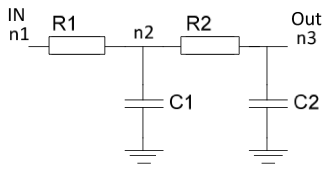
\includegraphics[scale=0.4]{pictures/tiefpass2ordnung}
  \end{figure}
  \item Stromgleichungen für Knoten $n_2$ und $n_3$ (out)
  \begin{gather*}
  0=(U_2-U_{in})\cdot \frac{1}{R_1}+(U_2-U_3)\cdot \frac{1}{R_2}+U_2\cdot s\cdot C_1\\
  0=(U_3-U_2)\cdot \frac{1}{R_2}+U_3\cdot s\cdot C_2\\
  U_2=R_2\cdot U_3\cdot (\frac{1}{R_2}+s\cdot C_2)\\
  \text{$U_2$ in oberer Gleichung eingesetzt und aufgelöst für
  $U_{out} /U_{in}$}\notag\\
  G_{p}(s)=\frac{1}{C_1\cdot R_1\cdot s+C_2\cdot R_1\cdot s+C_2\cdot R_2\cdot s+C_1\cdot C_2\cdot R_1\cdot R_2\cdot s^2+1}
  \end{gather*}
  Vergleich: Allgemeine Beschreibung von Tiefpass 2. Ordnung mit
  Verstärkung $A_0$, Kreisfrequenz $\omega_{0}$ und Güte Q
  \begin{align*}
  	T_{lp}(s)	&= \frac{A0}{\frac{s^2}{\omega_{0}^2}+\frac{s}{Q\omega_{0}}+1}\\
  	A0	 		&= 1 \\
  	\omega_{0}	&= \frac{1}{\sqrt{C_1\cdot C_2\cdot R_1\cdot R_2}}
  \end{align*}
  Güte berechnet mit Termen, die $s$ enthalten
  \begin{align*}
  	\frac{s}{Q\cdot \omega_{0}} &=C_1\cdot R_1\cdot s+C_2\cdot R_1\cdot s+C_2\cdot R_2\cdot s\\
  	Q 	&=\frac{\sqrt{C_1\cdot C_2\cdot R_1\cdot R_2}}{R_1\cdot (C_1+C_2)+C_2R_2}
  \end{align*}
  Passive RC-Filter können maximal Güte von 0.5 haben (2 identische reelle
  Pole) Filter höherer Güte benötigen Spulen oder Verstärker
\end{itemize}

\subsection{Sallen Key (Einfachmitkopplung)\hartl{517}}
\begin{figure}[ht]
	\centering
	\begin{subfigure}[b]{0.4\textwidth}
		\centering
		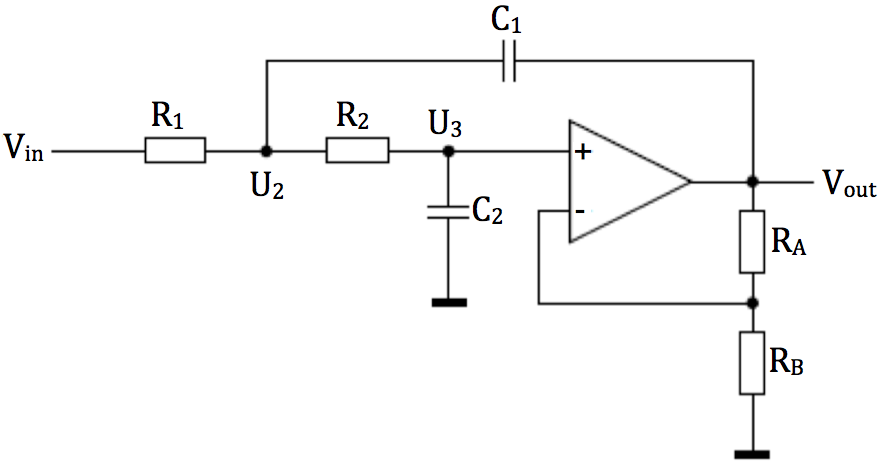
\includegraphics[scale=0.4]{./pictures/sallenkey.png}
		\caption{Standart Sallen Key}
	\end{subfigure}
	\qquad\qquad
	\begin{subfigure}[b]{0.4\textwidth}
		\centering
		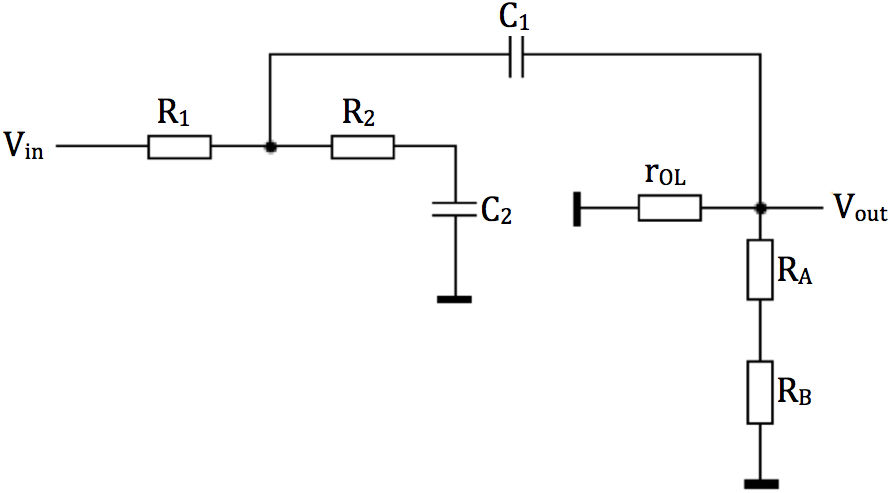
\includegraphics[scale=0.4]{./pictures/sallenkey2.png}
		\caption{für hohe Frequenzen}
	\end{subfigure}
\end{figure}
\begin{align*}
	0		&= (U_2-U_{in})\cdot \frac{1}{R_1}+(U_2-U_3)\cdot \frac{1}{R_2}+(U_2-U_{out})\cdot s\cdot C_1 \\
	0		&= (U_3-U_2)\cdot \frac{1}{R_2}+U_3\cdot s\cdot C_2\\
	U_{out}	&= U_{out}=G_0\cdot U_3 \\
	G_0		&= \frac{R_{A}+R_{B}}{R_{B}}\\
	G_{SK}	&= \frac{G0}{C_1\cdot C_2\cdot R_1\cdot R_2\cdot s^2+s\cdot [C_2\cdot (R_1+R_2)+C_1\cdot R_1\cdot (1-G_0)]+1}\\
	Q_{SK}	&= \frac{\sqrt{C_1\cdot C_2\cdot R_1\cdot R_2}}{C_2\cdot (R_1+R_2)+C_1\cdot R_1\cdot (1-G_0)}\\
	\omega_0 &= \frac{1}{\sqrt{C_1\cdot C_2\cdot R_1\cdot R_2}}
\end{align*}
Es wurden die folgenden Formelzeichen verwendet: $U_{out}$: Opamp Ausgangsspannung, $G_0$: ?, $Q_{SK}$: Güte des gesamten Schwingkreises, $G_{SK}$: ?,
$\omega_0$: Grenzfrequenz

\subsubsection{Sallen Key-Filter bei hohen Frequenzen}
\begin{itemize}
  \item Wenn der Opamp nicht mehr verstärkt
  \item $C_1$, $C_2$ wirken wie Kurzschlüsse
  \begin{equation*}
  \frac{V_{Out}}{V_{in}}=\frac{r_{OL}\parallel R_2\parallel
  (R_{A}+R_{B})}{R_1+r_{OL}\parallel R_2\parallel (R_{A}+R_{B})}\approx
  \frac{r_{OL}}{R_1+r_{OL}}
  \end{equation*}
  \item Folge: Sallen Key-Filter sind nicht geeignet für Systeme mit hohen
  Frequenzanteilen, z.B. PEM-DAC
\end{itemize}


\subsection{Multiple Feedback\hartl{522}}
\begin{figure}[!h]
	\centering
	\begin{subfigure}[b]{0.45\textwidth}
		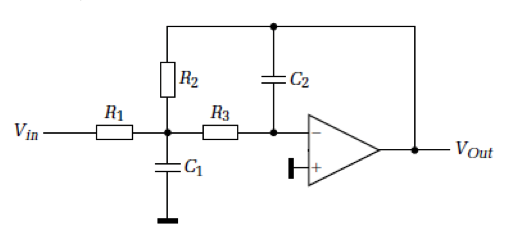
\includegraphics[scale=0.4]{./pictures/mulipleFeedback.png}
		\caption{Multiple Feedback}
	\end{subfigure}
	\begin{subfigure}[b]{0.45\textwidth}
		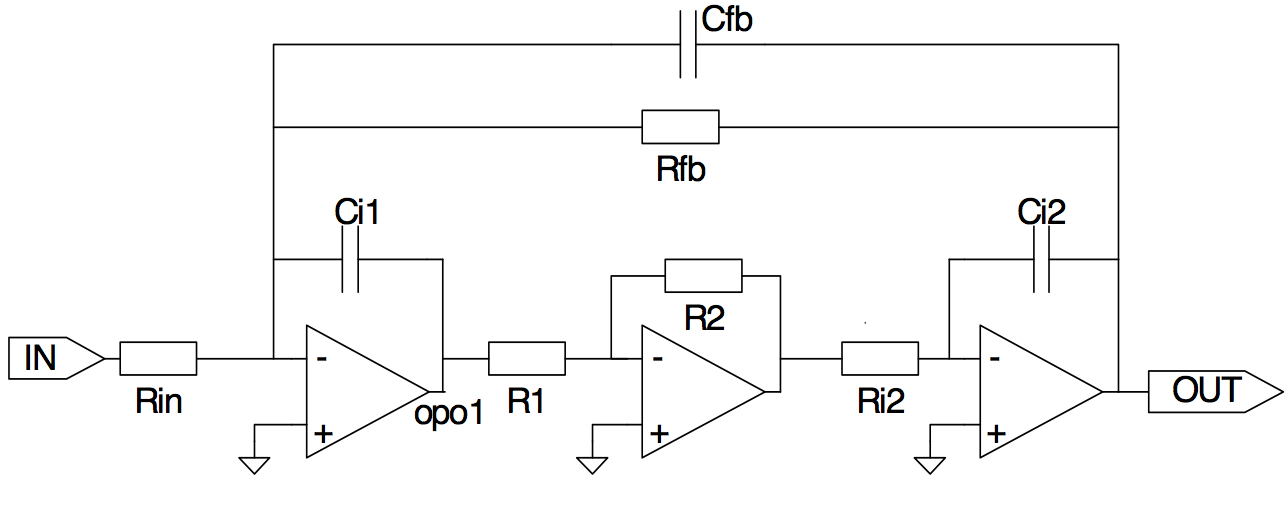
\includegraphics[scale=0.4]{./pictures/zustandsvariable.png}
		\caption{Zustandsvariable Filter}
	\end{subfigure}
\end{figure}
\begin{align*}
0			&=(U_2-U_{in})\cdot \frac{1}{R_1}+(U_2-U_{out})\cdot \frac{1}{R_2}+(U_2-U_3)\cdot \frac{1}{R_3}+U_2\cdot s\cdot C_1\\
0			&=(U_3-U_2)\cdot \frac{1}{R_3}+(U_3-U_{out})\cdot s\cdot C_2\\
			&\text{Opamp sorgt für }U_3=0\notag\\
G_{mf}(s)	&=\frac{G0}{1+C_2(R_2+R_3+R_3\cdot \frac{R_2}{R_1})\cdot s+C_1\cdot C_2\cdot R_2\cdot R_3\cdot s^s}\\
Q_{mf}		&=\frac{\sqrt{C_1\cdot C_2\cdot R_2\cdot R_3}}{C_2\cdot (R_2+R_3+R_3\cdot \frac{R_2}{R_1})}
\end{align*}
Die Güte wird v.a. eingestellt mit $C_2$ und $R_1$, grosse Güte für kleines
$C_2$ und grosses $R_1$. $C_2$ beeinflusst auch das Frequenzverhalten, $R_1$ die
Verstärkung.

\subsection{Zustandsvariablen-Filter}
\begin{align*}
	V{out}		&=-\frac{1}{s\cdot C_{i2}\cdot R_{i1}}\cdot V_{opo2}\\
	V_{opo2}	&=-\frac{R_2}{R_1}\cdot V_{opo1}\\
	V_{opo1}	&=\frac{-1}{s\cdot C_{i1}}\cdot (\frac{V_{in}}{R_{in}}+\frac{V_{out}}{R_{fb}}+s\cdot C_{fb}\cdot V_{out})\\
	G_{ss}(s)	&=\frac{-\frac{R_{fb}}{R_{in}}}{C_{i1}\cdot C_{i2}\cdot R_{i1}\cdot R_{fb}\cdot \frac{R_1}{R_2}\cdot s^2+C_{fb}\cdot R_{fb}\cdot s+1}\\
	\omega_{0}	&=\frac{1}{\sqrt{C_{i1}\cdot C_{i2}\cdot R_{i1}\cdot R_{fb}\cdot \frac{R_1}{R_2}}}\\
	A_{0}		&=-\frac{R_{fb}}{R_{in}}\\
	Q			&=\frac{\sqrt{C_{i1}\cdot C_{i2}\cdot R_{i1}\cdot R_{fb}\cdot \frac{R_1}{R_2}}}{C_{fb}\cdot R_{fb}}
\end{align*}
D.h. mit dieser Topologie sind alle 3 Parameter frei wählbar!
\begin{enumerate}
  \item $\omega_{0}$ mit $C_{i1}$, $C_{i2}$, $R_{fb}$, $R_{i2}$, $R_1$, $R_2$
  \item Q mit $C_{fb}$
  \item $A_0$ mit $R_{in}$
\end{enumerate}


